\section{Method}

\subsection*{Rationale for Survey Imputation with LLMs}

There are many advanced methods for survey imputations. However, we aim to explore whether Large Language Models (LLMs) can provide more insights into voters' thought processes while imputing their survey responses. If an LLM can predict party affiliations based on given statements, it might reveal aspects of human reasoning that other survey imputation methods cannot, especially since traditional methods do not inquire about the rationale behind choices.

\subsection*{Prompt Engineering}

We can consider various potential directions such as fine-tuning, instruction tuning, representation engineering, and prompt engineering. As a basic initial step, we focus on prompt engineering to maximize the potential of our model by ensuring the quality of prompts.

\subsection*{Methodology}

Our study uses survey responses from the European Social Survey (ESS) related to political interests and socio-political orientations to predict party affiliations within the same survey. We employ two models: the first model processes survey responses for input variables and generates \textit{Statements}, which are normal human-like speeches rather than discrete survey numbers. The second model uses these statements to predict party affiliations by analyzing what someone who made those statements might think about the target survey variable. We evaluate the performance by employing accuracy metrics, using ESS data as the gold standard.

\subsection*{Model Choice}

For our research, LLaMA 2 is the optimal choice due to its advanced features and suitability for handling complex natural language tasks. The ESS data encompasses a wide range of social variables, including political interest, socio-political orientations, and party allegiance, which are crucial for our study on predicting political affiliations. LLaMA 2's transformer architecture and fine-tuning with reinforcement learning from human feedback (RLHF) enable it to generate coherent, contextually appropriate text from open-ended survey responses. This aligns well with our need to convert survey responses into natural statements and then predict political orientations based on these statements. Furthermore, LLaMA 2's flexibility in fine-tuning on various platforms enhances its adaptability to our specific research requirements, ensuring accurate and nuanced predictions. This approach leverages the comprehensive nature of the ESS data and the advanced capabilities of LLaMA 2, as discussed in recent literature on state-of-the-art language models.

\begin{figure}[h]
    \centering
    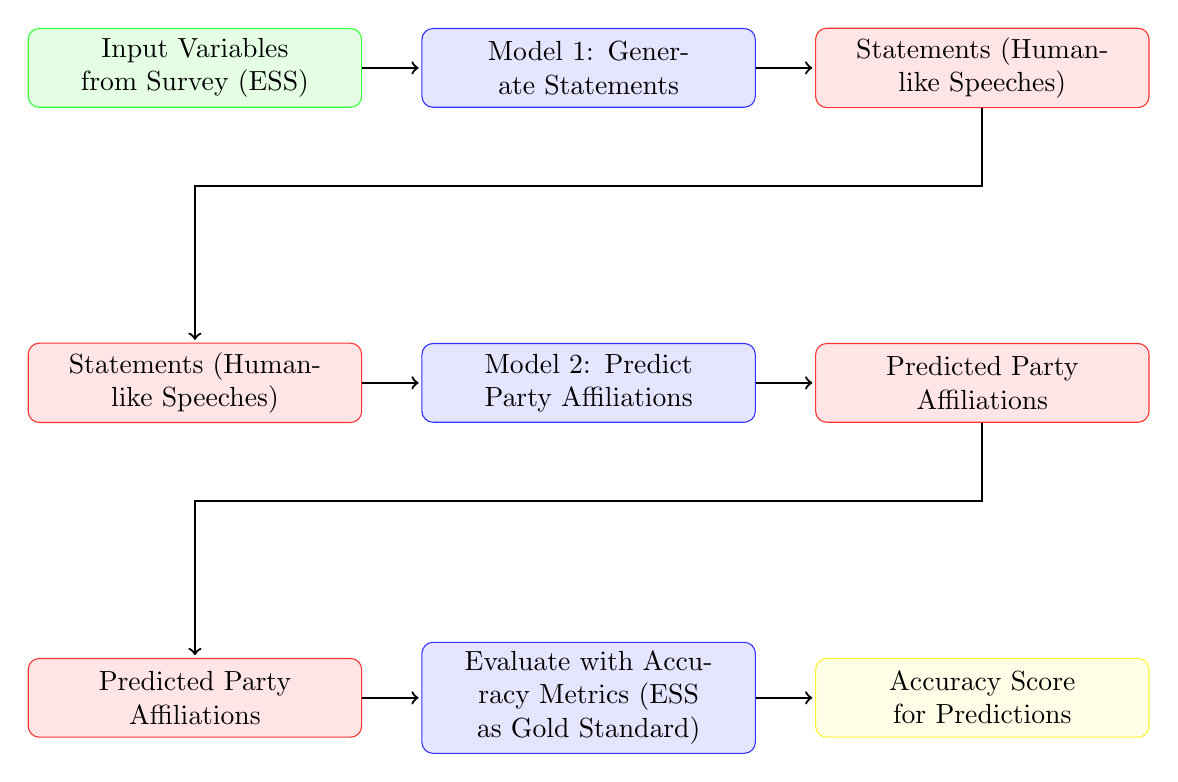
\begin{tikzpicture}[
      node distance=2.5cm and 2.5cm,
      every node/.style={fill=blue!10, rectangle, rounded corners, draw=blue!80, align=center, text width=4cm, minimum height=1cm},
      input/.style={fill=green!10, rectangle, rounded corners, draw=green!80},
      output/.style={fill=red!10, rectangle, rounded corners, draw=red!80},
      finaloutput/.style={fill=yellow!10, rectangle, rounded corners, draw=yellow!80},
      evaluation/.style={fill=blue!10, rectangle, rounded corners, draw=blue!80},
      every arrow/.style={draw, thick, ->, shorten >=1pt},
    ]

    % First row
    \node[input] (input1) {Input Variables from Survey (ESS)};
    \node (model1) [right of=input1, xshift=2.5cm] {Model 1: Generate Statements};
    \node[output] (output1) [right of=model1, xshift=2.5cm] {Statements (Human-like Speeches)};

    % Second row
    \node[output] (output1_dup) [below of=input1, yshift=-1.5cm] {Statements (Human-like Speeches)};
    \node (model2) [right of=output1_dup, xshift=2.5cm] {Model 2: Predict Party Affiliations};
    \node[output] (output2) [right of=model2, xshift=2.5cm] {Predicted Party Affiliations};

    % Third row
    \node[output] (output2_dup) [below of=output1_dup, yshift=-1.5cm] {Predicted Party Affiliations};
    \node[evaluation] (final_evaluation) [right of=output2_dup, xshift=2.5cm] {Evaluate with Accuracy Metrics (ESS as Gold Standard)};
    \node[finaloutput] (accuracy_score) [right of=final_evaluation, xshift=2.5cm] {Accuracy Score for Predictions};

    % Arrows
    \draw [every arrow] (input1) -- (model1);
    \draw [every arrow] (model1) -- (output1);
    \draw [every arrow] (output1) -- ++(0, -1.5) -| (output1_dup);
    \draw [every arrow] (output1_dup) -- (model2);
    \draw [every arrow] (model2) -- (output2);
    \draw [every arrow] (output2) -- ++(0, -1.5) -| (output2_dup);
    \draw [every arrow] (output2_dup) -- (final_evaluation);
    \draw [every arrow] (final_evaluation) -- (accuracy_score);

    \end{tikzpicture}
    \caption{The diagram illustrates the research methodology for survey imputation using Large Language Models (LLMs). Input variables from the ESS survey are transformed into human-like statements by Model 1. These statements are then used by Model 2 to predict party affiliations. The predicted affiliations are evaluated against the gold standard using accuracy metrics, with the final accuracy score for the predicted party affiliations being calculated.}
\end{figure}
